\chapter{Cuadrados Mínimos}
Consideremos el problema
$$
\Ab\xb=\bb
$$
con $\Ab\in \Rmn$. La existencia de soluciones de este problema equivale a que 
$\bb\in \langle \ab_1,  \ab_2,\cdots , \ab_n\rangle$ ($\ab_{i}$ son las columnas de $\Ab$) y en ese caso la unicidad depende de que el conjunto 
$\{ \ab_1,  \ab_2,\cdots , \ab_n\}$ sea $l.i.$. 

En el caso en que $\bb\notin \langle  \ab_1,  \ab_2,\cdots , \ab_n\rangle$
podemos intentar minimizar el residuo
$$
\rb=\bb-\Ab\xb
$$
Para eso nos conviene usar una norma: la norma $2$  es la mas adecuada como veremos en breve.

El problema es entonces,  hallar $\xb\in \Rn$ tal que
$$
\|\Ab\xb-\bb\|_2=min_{\zb\in \Rn}\|\Ab\zb-\bb\|_2
$$
o el equivalente 
hallar $\xb\in \Rn$ tal que
$$
\|\Ab\xb-\bb\|_2^2=min_{\zb\in \Rn}\|\Ab\zb-\bb\|_2^2
$$
el enfoque tradicional (fuera del álgebra lineal numérica) es buscar una ecuación para el punto crítico $\xb$ como minimizante. 

Eso equivale a anular el gradiente de la función $F:\Rn\to \R$, $F(\zb)=\|\Ab\zb-\bb\|_2^2$, es decir
$$
0=\frac{\partial F}{\partial z_k}|_{\xb}=\sum_{i=1}^m\frac{\partial \left( [\Ab\zb-\bb \right]_i)^2}{\partial z_k}|_{\xb}=
$$
$$
\sum_{i=1}^m\frac{\partial \left( \sum_{j=1}^na_{ij}z_j-b_i \right)^2}{\partial z_k}|_{\xb}=2\sum_{i=1}^m\left( \sum_{j=1}^na_{ij}x_j-b_i\right)a_{ik}
$$
La validez de esta identidad para todo $1\le k\le n$ dice que 
$$
\Ab^T(\Ab\xb-\bb)=\cero
$$

Dicho de otro modo
$$
\Ab^T\Ab\xb=\Ab^T\bb
$$
estas se llaman las ecuaciones normales. 

A pesar de su popularidad esta no siempre es la mejor manera de calcular $\xb$.


Desde esas ecuaciones podemos deducir cuando habrá solución única de nuestro problema: si las columnas de $A$ son $l.i.$ entonces $\Ab^T\Ab\xb=\cero$ implica 
$$
0=(\Ab^T\Ab\xb)^T\xb=(\Ab\xb)^T\Ab\xb=\|\Ab\xb\|_2^2,
$$
es decir $\Ab\xb=\cero$ y así $\xb=\cero$ por ser las columnas de $\Ab$ $l.i.$, por lo que el núcleo de $\Ab^T\Ab$ es trivial.

Observemos que en este caso $\Ab^T\Ab\in \Rnn$ resulta \emph{simétrica definida positiva}.
En particular podemos resolver el sistema usando Cholesky a un costo $\sim mn^2+ \frac{1}{3}n^{3}$

En gran parte de las aplicaciones $m >> n$ y las columnas de $\Ab$ son $l.i.$ lo cual muestra el éxito relativo de las ecuaciones normales.
\section{Interpolación Polinomial}
Un caso tradicional de uso de cuadrados mínimos es en aproximación polinomial. 

El problema de la interpolación consiste en lo siguiente: dados $n+1$ pares de puntos $\{(x_{0},y_{0}),(x_{1},y_{1})\cdots ,(x_{n},y_{n})\}\subset \Kn$ hallar un polinomio $p_{n}(x)$ de grado a lo sumo $n$ tal que $p_{n}(x_{i})=y_{i}$.


Con los $x_{i}\neq x_{j}$ este problema siempre tiene solución única gracias a las siguientes observaciones.


 
 Se propone $p_{n}(x)=a_{0}+ a_{1}x+\cdots +a_{n-1}x^{n-1} +a_{n}x^{n}$ y se hace $p_{n}(x_{i})=y_{i}$ para todo $0\le i\le n$ que conduce a un sistema lineal con matriz de Vandermonde $V[x_0,x_1,\cdots,x_n]$
 $$
 \begin{pmatrix}
 1&x_{0}&x_{0}^{2}&\cdots &x_{0}^{n}\\
 1&x_{1}&x_{1}^{2}&\cdots &x_{1}^{n}\\
 \vdots&\vdots&\vdots&\cdots&\vdots\\
 1&x_{n}&x_{n}^{2}&\cdots &x_{n}^{n}\\
 \end{pmatrix}
 \begin{pmatrix}
 a_{0}\\
 a_{1}\\
 \vdots\\
 a_{n}
 \end{pmatrix}=
 \begin{pmatrix}
y_{0}\\
 y_{1}\\
 \vdots\\
 y_{n}
 \end{pmatrix}.
 $$
 Se tiene
 $$
 \det V[x_0,x_1,\cdots,x_n]=\Pi_{0\le i<j\le n}(x_j-x_i).
 $$
 (La demo mas corta que conozco...) 
 
 Vale en $2\times 2$ y sale por inducción: supongo que vale hasta $n-1$. 
 
 LLamo
 $p_n(x)=\det V[x_0,x_1,\cdots,x_{n-1},x]$, claramente es polinomio y tiene grado $n$, su coeficiente principal es (desarrollo por la primera fila y uso hipótesis inductiva) $\det V[x_0,x_1,\cdots,x_{n-1}]=\Pi_{0\le i<j\le n-1}(x_j-x_i)$.
 
  Ademas las raíces de $p_n(x)$ son exactamente $x_0,x_1,\cdots, x_{n-1}$, luego se escribe como
 $$
 p_n(x)=\Pi_{0\le i<j\le n-1}(x_j-x_i)\Pi_{k=0}^{n-1}(x-x_k),
 $$
 evaluando en $x=x_n$ se obtiene el resultado mencionado. 
 
 En particular el problema de interpolación tiene solución única...

Hay otros enfoques... Lagrange
$$
L_i(x)=\frac{\Pi_{0\le j\le n, j\neq i}(x-x_j)}{\Pi_{0\le j\le n, j\neq i}(x_i-x_j)}
$$
 $$
 L_i(x_j)=\delta_i^j
 $$
 $$
 p_n(x)=\sum_{i=0}^ny_iL_i(x).
 $$
 La unicidad sale aparte...

 Problemas de la interpolación:
 
 \begin{figure}
\centering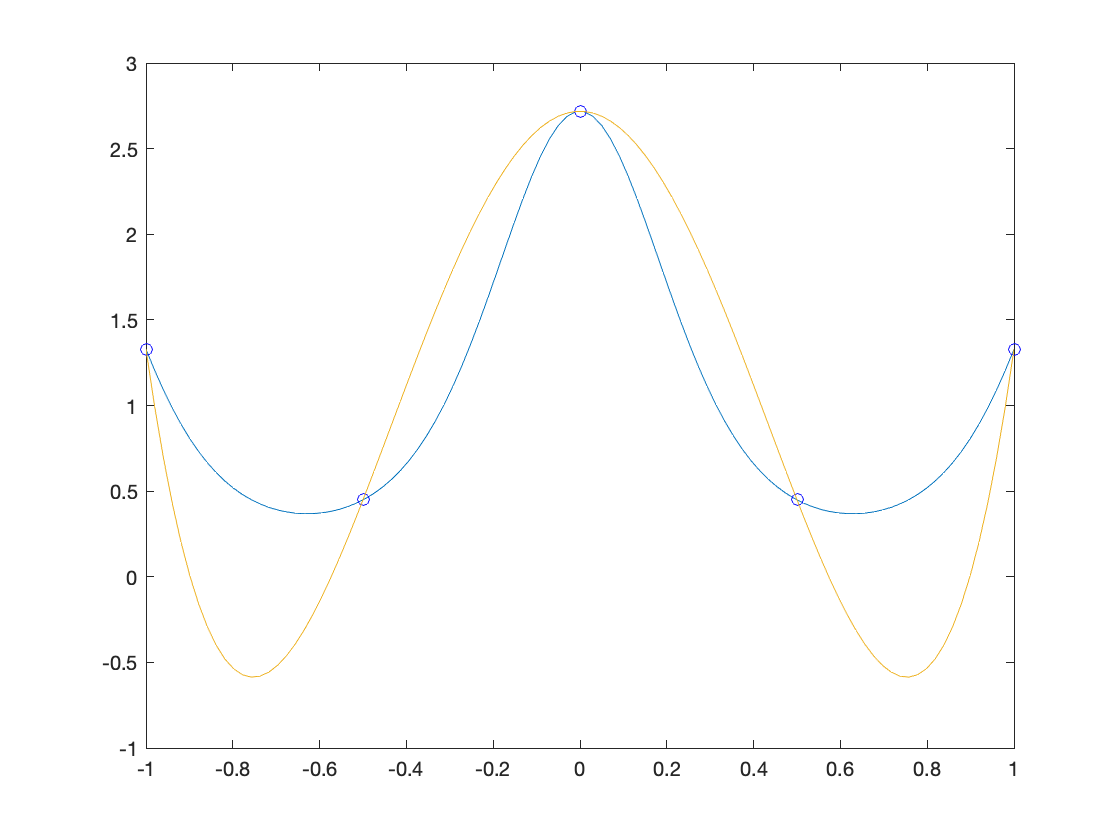
\includegraphics[width=0.4\linewidth]{interp5.png}
\end{figure}


\begin{figure}
\centering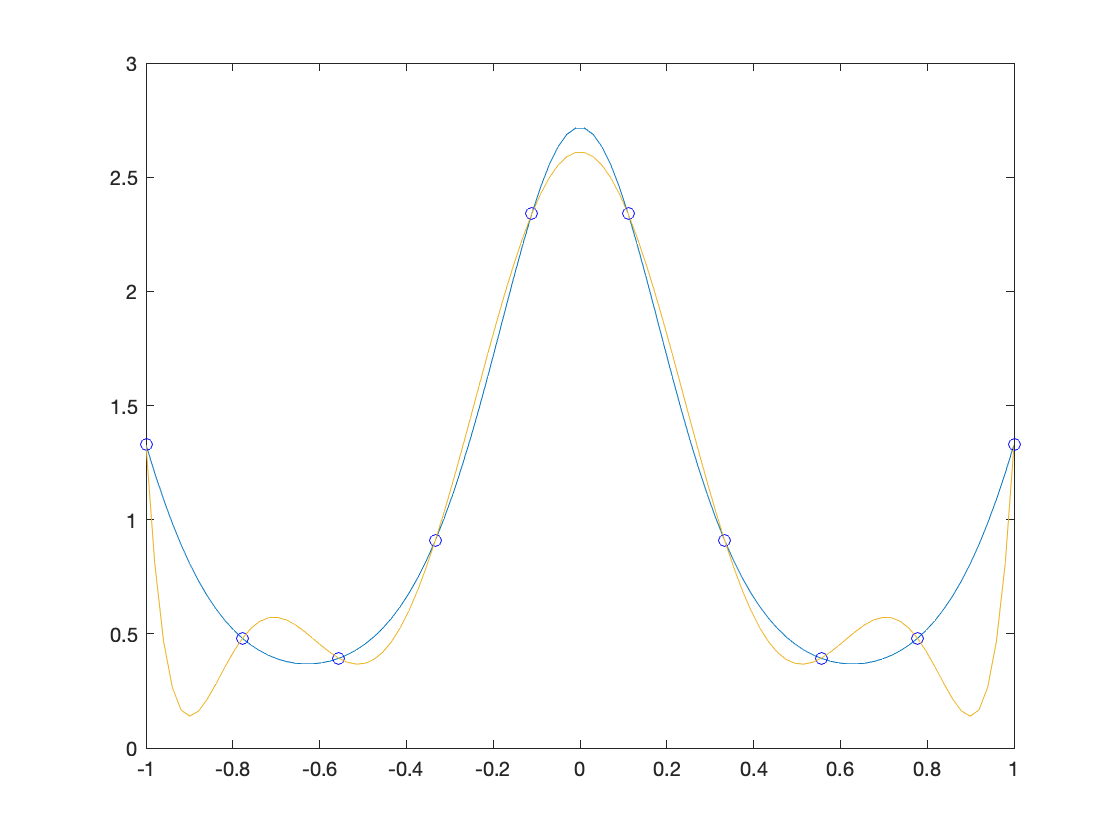
\includegraphics[width=0.4\linewidth]{interp10.png}
\end{figure}

\begin{figure}
\centering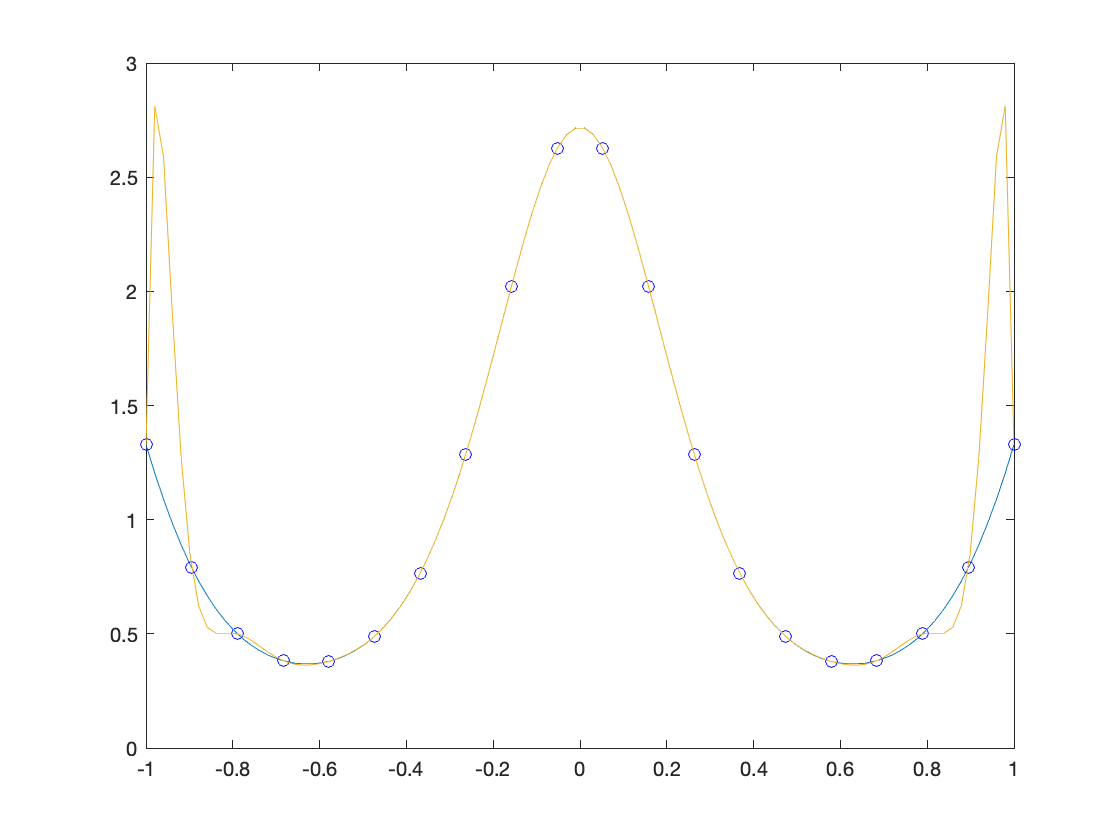
\includegraphics[width=0.4\linewidth]{interp20.png}
\end{figure}


 \begin{figure}
\centering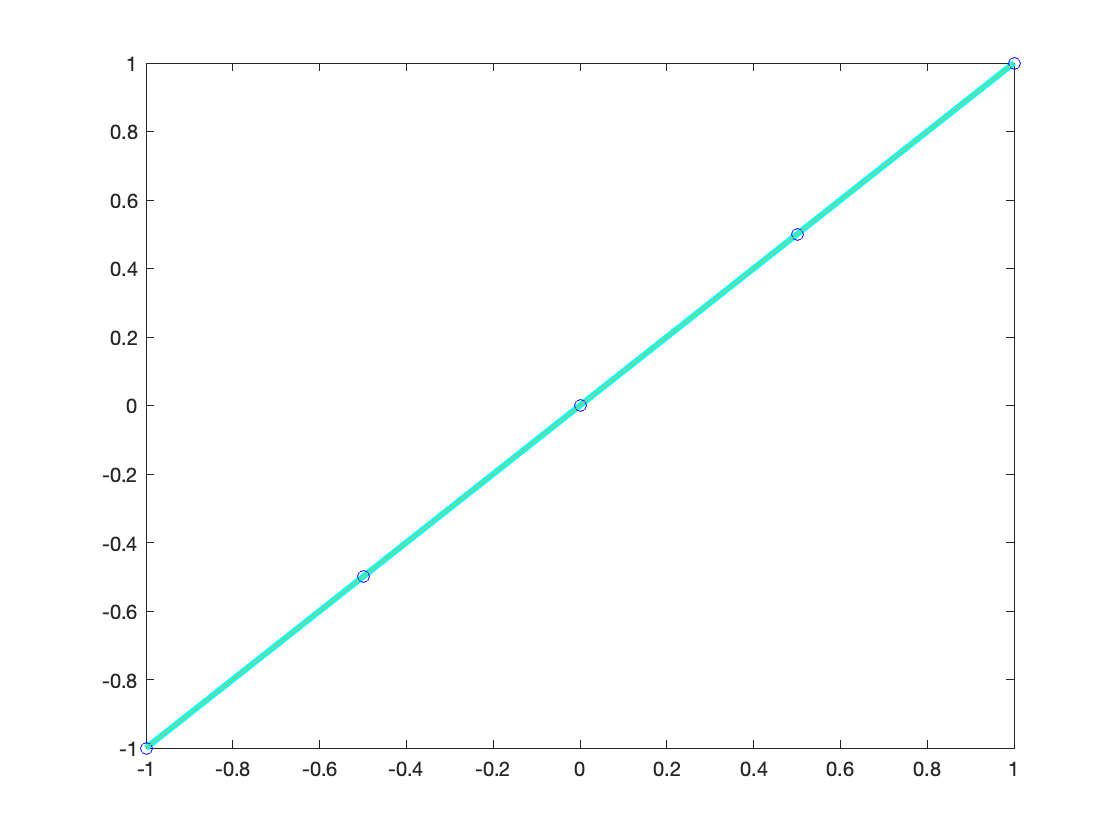
\includegraphics[width=0.4\linewidth]{recta5.png}
\end{figure}

 
 \begin{figure}
\centering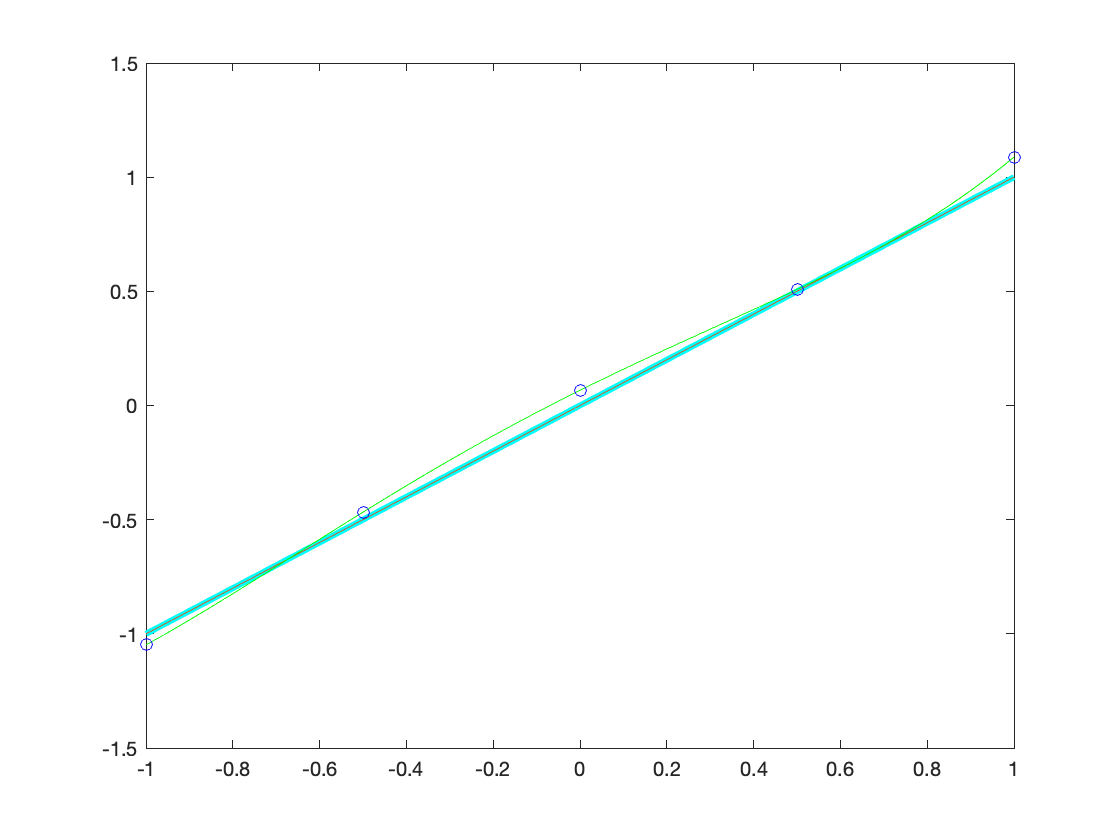
\includegraphics[width=0.4\linewidth]{linea5rand.png}
\end{figure}

\begin{figure}
\centering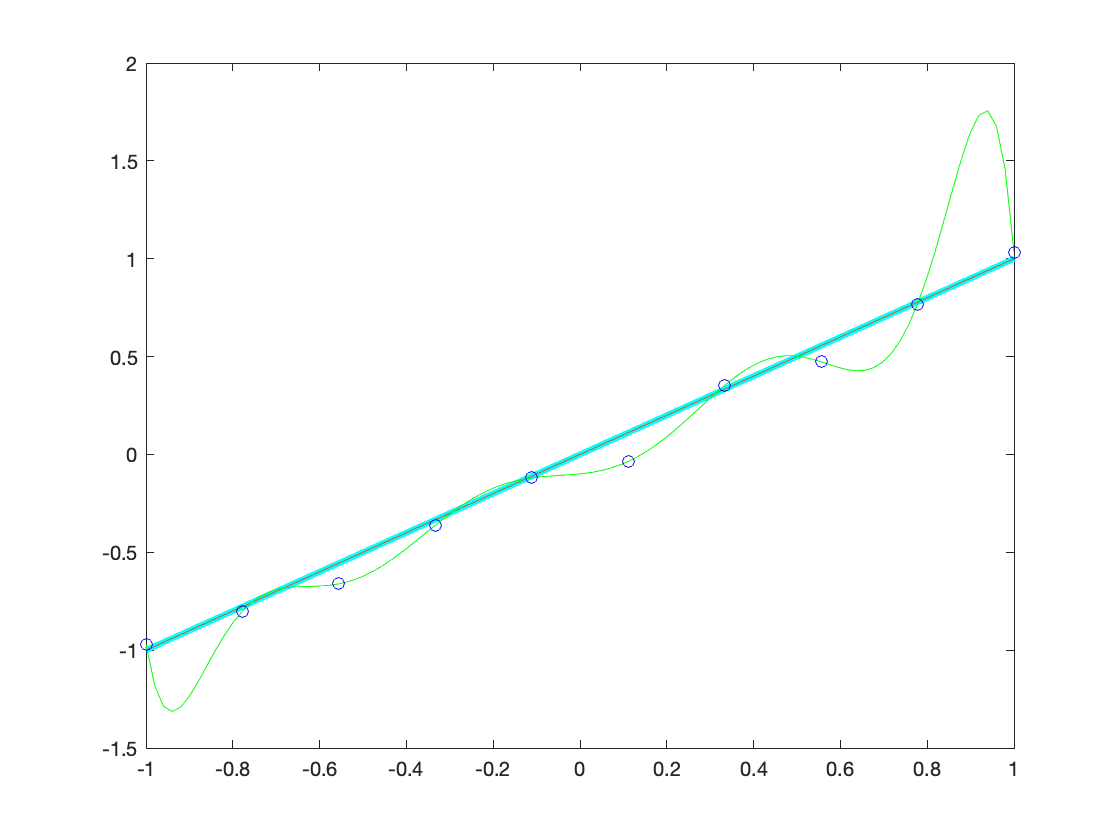
\includegraphics[width=0.4\linewidth]{linea10rand.png}
\end{figure}

\begin{figure}
\centering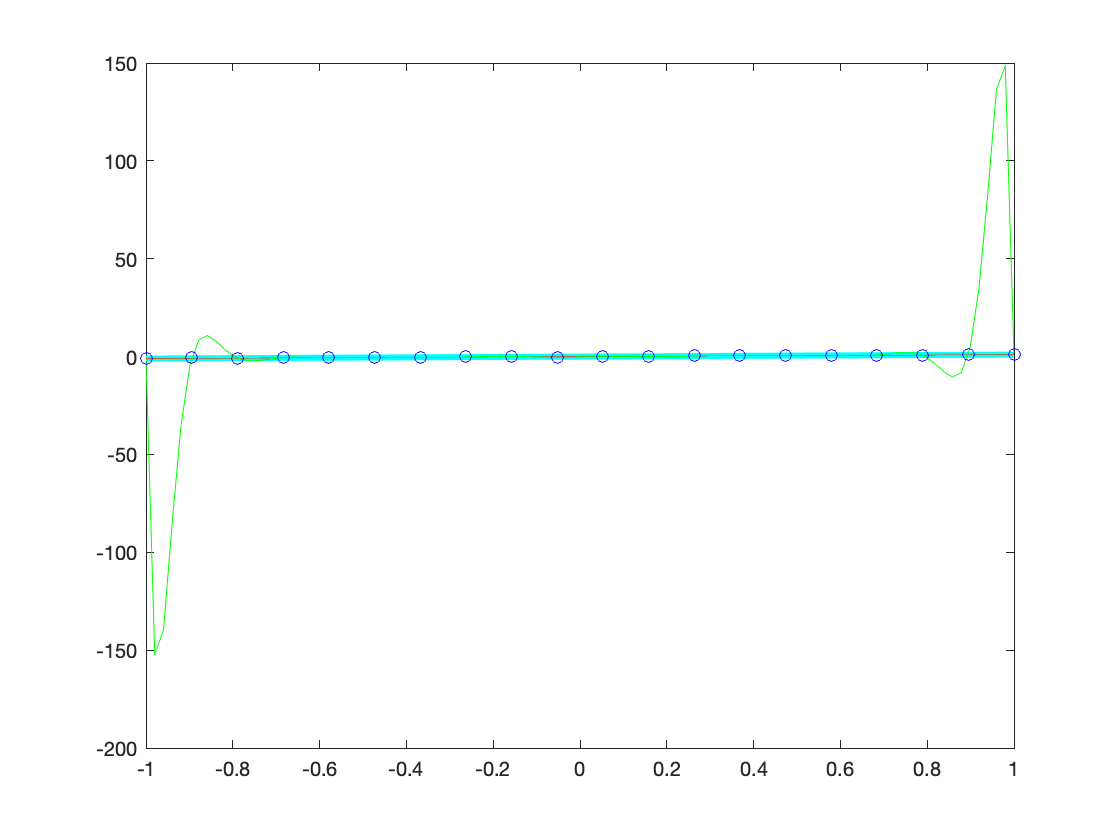
\includegraphics[width=0.4\linewidth]{linea20rand.png}
\end{figure}

La teoría anterior se aplica igual las matrices de Vandermonde son ($m>>n$)
 $$
 \begin{pmatrix}
 1&x_{0}&x_{0}^{2}&\cdots &x_{0}^{n}\\
 1&x_{1}&x_{1}^{2}&\cdots &x_{1}^{n}\\
 \vdots&\vdots&\vdots&\cdots&\vdots\\
 \vdots&\vdots&\vdots&\cdots&\vdots\\
  \vdots&\vdots&\vdots&\cdots&\vdots\\
 1&x_{m}&x_{m}^{2}&\cdots &x_{m}^{n}\\
 \end{pmatrix}
$$
notar que las columnas son $l.i.$ porque las primeras $n+1$ filas forman una matriz de Vandermonde 
cuadrada invertible.

Si hacemos $n=1$ 
$$
 \begin{pmatrix}
 1&x_{0}\\
 1&x_{1}\\
 \vdots&\vdots\\
 1&x_{m}\\
 \end{pmatrix}
 \begin{pmatrix}
 a_{0}\\
 a_{1}
 \end{pmatrix}=
 \begin{pmatrix}
y_{0}\\
 y_{1}\\
 \vdots\\
 y_{m}
 \end{pmatrix}.
 $$
las ecuaciones normales conducen a la tradicional expresión
$$
\begin{pmatrix}
1&\frac{1}{m+1}\sum_{i=0}^mx_i\\
\frac{1}{m+1}\sum_{i=0}^mx_i&\frac{1}{m+1}\sum_{i=0}^mx_i^2
\end{pmatrix}
\begin{pmatrix}
 a_{0}\\
 a_{1}
 \end{pmatrix}=
 \begin{pmatrix}
\frac{1}{m+1}\sum_{i=0}^my_i\\
 \frac{1}{m+1}\sum_{i=0}^mx_iy_i
 \end{pmatrix}.
$$ 

 \begin{figure}[h]
\centering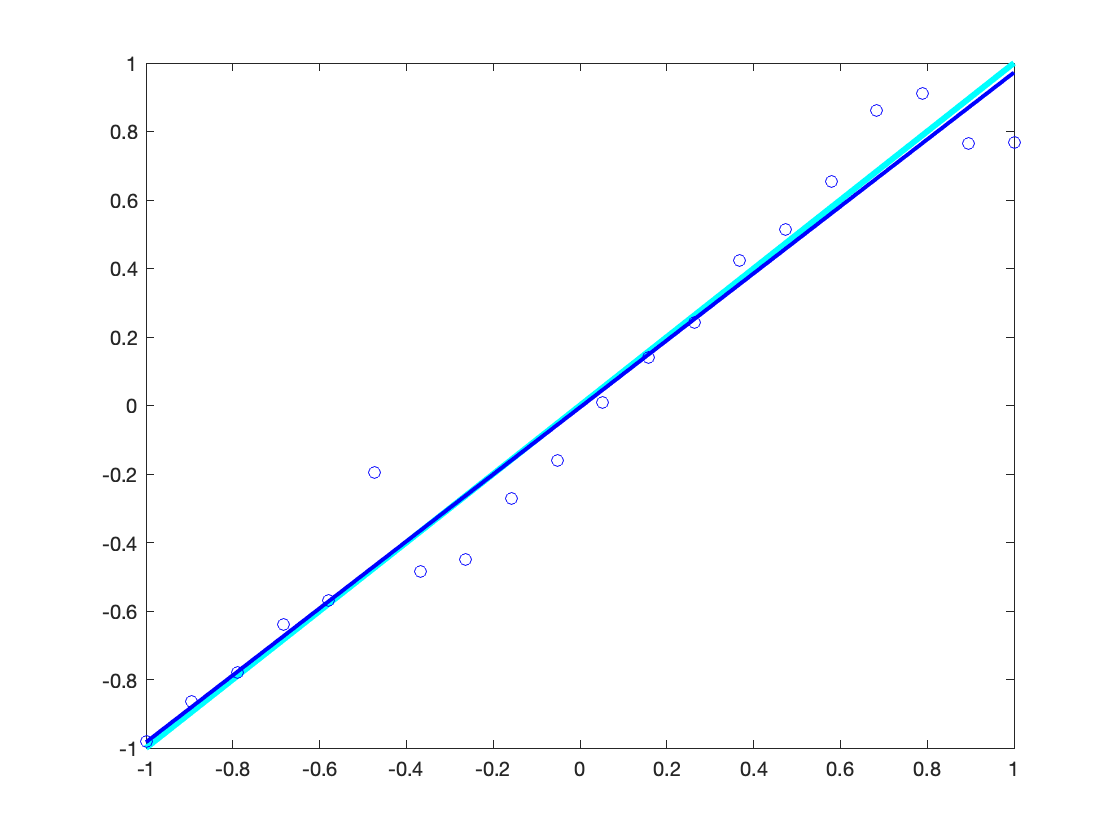
\includegraphics[width=0.4\linewidth]{minimosminimos.png}
\end{figure}

 Intuitivamente si
 $$
 \Ab=\Ub\Sigma\Vb^*
 $$
 y $\Ab\in \R^{m\times n}$, vimos que puede definirse la condición de $\Ab$ como $\frac{\sigma_1}{\sigma_n}$. Si hacemos $\Ab^T\Ab=\Vb\Sigma^2\Vb^*$ vemos que en las ecuaciones normales la condición de la matriz final empeora $\kappa(\Ab^T\Ab)=\left(\frac{\sigma_1}{\sigma_n}\right)^2$. 

Problema revisitado
\begin{figure}[h]
\centering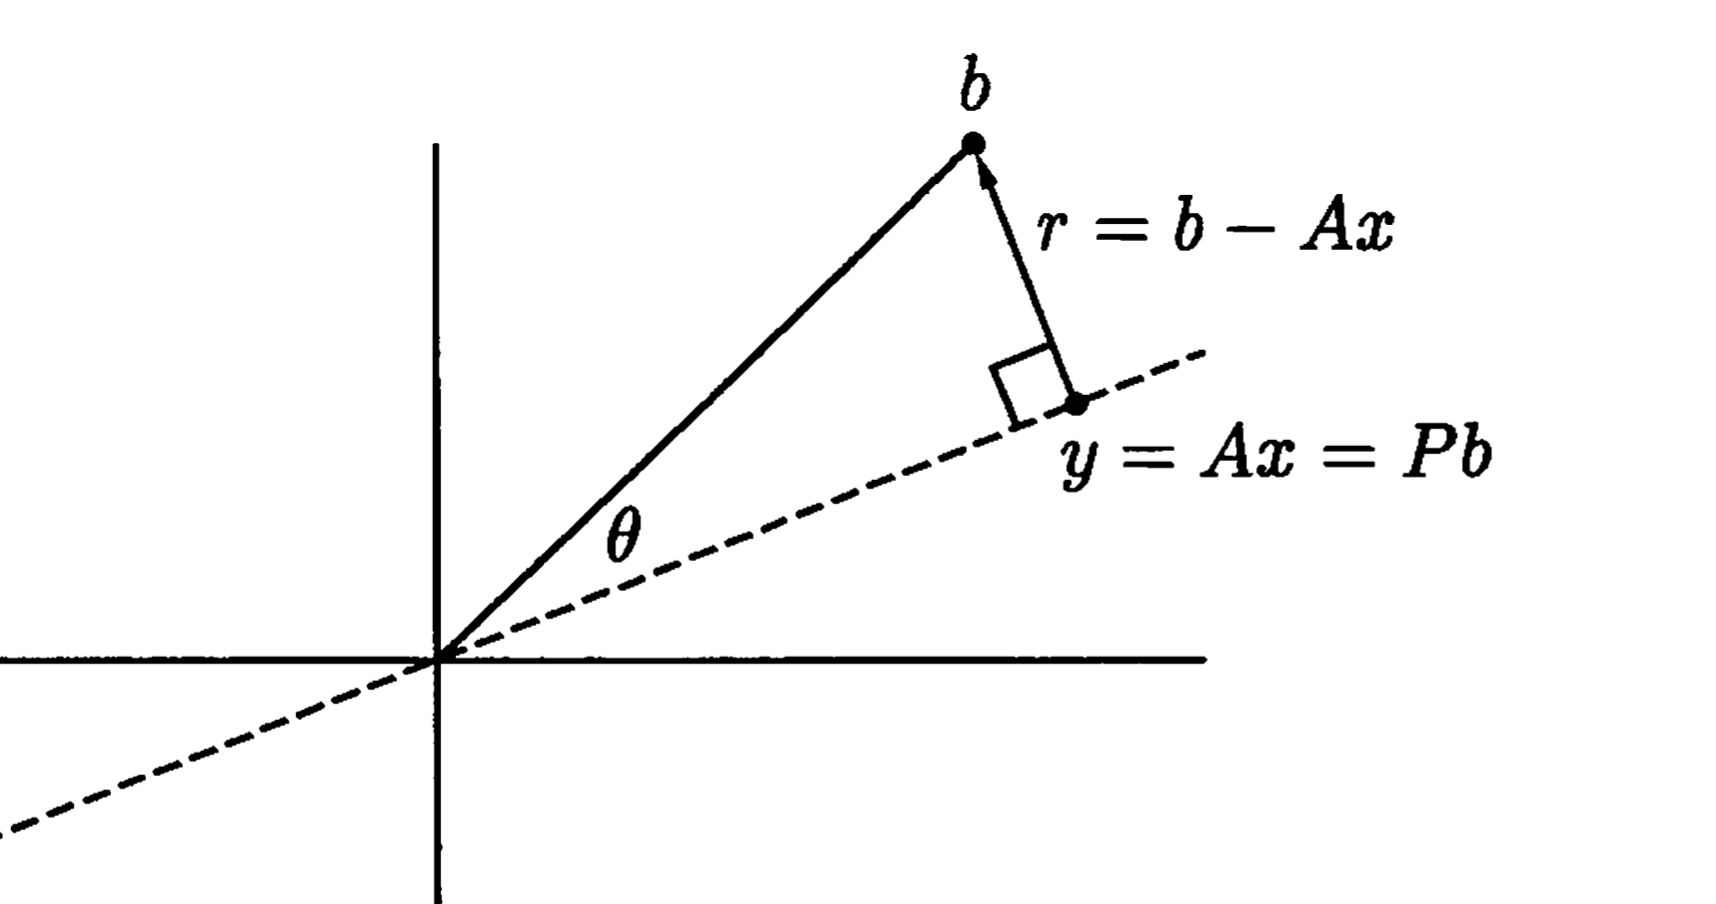
\includegraphics[width=0.4\linewidth]{cuadmin.png}
\end{figure}

El gráfico sugiere otro enfoque: construir el proyector $P$ sobre la imagen de $\Ab$. Esto es , si $\{\qb_1,\cdots,\qb_n\}$ es una base ortonormal de $\mathcal{S}=Im(\Ab)$ tenemos
$$
P_{\mathcal{S}}\bb=\Qb\Qb^*\bb
$$ 
donde 
$$
\Qb=
\begin{pmatrix}
\qb_1|\qb_2|\cdots |\qb_n
\end{pmatrix}
$$
La obtención de $\Qb\in \R^{m\times n}$ puede hacerse con la factorización $QR$, es decir
$$
\Ab=\Qb\Rb
$$
con $\Rb\in \R^{n\times n}$ triangular superior.  

Escribimos  
$$
\Qb\Rb\xb=\Ab\xb=P_{\mathcal{S}}\bb=\Qb\Qb^*\bb
$$
es decir que basta resolver
$$
\Rb\xb=\Qb^*\bb
$$
Este algoritmo es mas estable que el de las ecuaciones normales su costo esta gobernado por $QR$  que es 
$\sim 2mn^2-\frac13n^3$.
Volvemos a las ecuaciones normales: supongamos que $\Ab\in \R^{m\times n}$, $m>>n$, rango $n$  (columnas l.i.): debemos resolver
$$
\Ab^t\Ab\xb=\Ab^t\bb
$$
si escribimos $\Ab=\Ub\Sigma\Vb^*$, tenemos
$$
\Vb\Sigma^t\Sigma\Vb^t\xb=\Ab^t\Ab\xb=\Ab^t\bb=\Vb\Sigma^t\Ub^t\bb
$$

Como 
$$\Sigma=
\begin{pmatrix}
\sigma_1&0&0&\cdots &0\\
0&\sigma_2&0&\cdots &0\\
0&0&0&\cdots&\sigma_n\\
0&0&0&\cdots&0\\
\vdots&\vdots&\vdots&\cdots&\vdots\\
0&0&0&\cdots&0
\end{pmatrix}
$$
y
$$\Sigma^t=
\begin{pmatrix}
\sigma_1&0&0&\cdots &0&\cdots&0\\
0&\sigma_2&0&\cdots &0&\cdots&0\\
0&0&0&\cdots&\sigma_n&\cdots&0
\end{pmatrix}
$$
tenemos

$$
\Sigma^t\Sigma=
\begin{pmatrix}
\sigma_1^2&0&0&\cdots &0\\
0&\sigma_2^2&0&\cdots &0\\
0&0&\ddots&0&0\\
0&0&\ddots&0&\sigma_n^2
\end{pmatrix}
$$
entonces

$$
\xb=
\Vb
\begin{pmatrix}
\sigma_1^{-1}&0&0&\cdots &0&\cdots&0\\
0&\sigma_2^{-1}&0&\cdots &0&\cdots&0\\
0&0&0&\cdots&\sigma_n^{-1}&\cdots&0
\end{pmatrix}
\Ub^t\bb
$$
o sea
$$
\xb=
\Ab^+\bb
$$
y la pseudoinversa funciona como "inversa".

En general en el caso $m>>n$ podríamos tener rango menor a $n$ (digamos $r<n$).

Recordemos que de $\Ab=\Ub\Sigma\Vb^t$, tenemos que para $1\le i\le r$
$$
\Ab\vb_i=\Ub\Sigma\Vb^t\vb_i=\Ub\Sigma\eb_i=\Ub\sigma_i\eb_i=\sigma_i\Ub_i
$$
y 
$$
\Ab\vb_i=\cero
$$
si $r<i\le n$. 


Luego $ker(\Ab)=\langle \vb_{r+1},\cdots,\vb_n\rangle $ y
$Im(\Ab)=\langle \ub_1,\cdots,\ub_r\rangle$.

De hecho
$$
\Ab^+\Ab=
\vb\Sigma^+\Sigma\vb^t=
\vb\begin{pmatrix}
1&0&\cdots &0&\cdots &0\\
0&1&\cdots &0&\cdots &0\\
\vdots&\vdots&&\vdots&&\vdots\\
0&0&\cdots &1&\cdots &0\\
0&0&\cdots &0&\cdots &0\\
\vdots &\vdots&\vdots &\vdots &\vdots\\

0&0& \cdots &0&\cdots &0\\

\end{pmatrix}
\vb^t
$$

Queremos estudiar $\Ab^+\bb$ en este caso.

El producto 
$$
\Ub^t\bb=
\begin{pmatrix}
\ub_1^t\bb\\
\ub_2^t\bb\\
\vdots\\
\ub_m^t\bb
\end{pmatrix}
$$
así
$$
\Sigma^+\Ub^t\bb=
\begin{pmatrix}
\sigma_1^{-1}(\ub_1^t\bb)\\
\sigma_2^{-1}(\ub_2^t\bb)\\
\vdots\\
\sigma_r^{-1}(\ub_r^t\bb)\\
0\\
\vdots\\
0
\end{pmatrix} \in \R^{n\times 1}
$$

entonces
$$
\xb=\Vb\Sigma^+\Ub^t\bb=
\sum_{j=1}^r\sigma_j^{-1}(\ub_j^t\bb)\vb_j
$$
Chequeamos
$$
\Ab\xb=\sum_{j=1}^r\sigma_j^{-1}(\ub_j^t\bb)\Ab\vb_j=\sum_{j=1}^r(\ub_j^t\bb)\ub_j=P_{Im(A)}\bb
$$
y vemos que es solución del problema de cuadrados mínimos.

Si hubiera otro $\tilde \xb$ tal que $\Ab\tilde\xb=P_{Im(A)}\bb$ entonces
$$
\Ab(\tilde\xb-\xb)=\cero
$$
luego
$$
\tilde\xb-\xb=\sum_{j=r+1}^n\alpha_j\vb_j
$$
$$
\tilde\xb= \xb+\sum_{j=r+1}^n\alpha_j\vb_j
$$

como $\xb\perp \vb_j$ para todo $r+1\le j\le n$
$$
\|\tilde\xb\|^2=\tilde\xb^t\tilde\xb=\xb^t\xb+\sum_{j=r+1}^n|\alpha_j|^2
$$
i.e.
$$
\|\xb\|<\|\tilde\xb\|
$$
la pseudoinversa da la solución de menor norma $2$.
 
 \centerline {Relación con regularización:} 

En el caso de rango $r<n$ (o muy mal condicionado) también se puede pensar el problema del modo siguiente: minimizar
 $$
 F(\zb)=\|\Ab\zb-\bb\|^2+\alpha^2\|\zb\|^2
 $$
 y luego hacer $\alpha\to 0$. 
 
 \begin{itemize}
 \item  El término se elige $\alpha^2$ para garantizar signo
\item La expresión: $\alpha^2\|\zb\|^2$ se denomina penalización (se penalizan valores grandes de  $\|\zb\|$.
\item Para cada $\alpha$ tenemos una solución: la denotamos $\xb_\alpha$.
 \end{itemize}
 Decimos que 
 $$
 \xb_\alpha\to \xb \, \mbox{solución dada por}\, \Ab^+
 $$
 En efecto: para el mínimo de $F$ se tiene 
 $$
 2(\Ab^t(\Ab\xb_\alpha-\bb)+\alpha^2\xb_\alpha)=\cero
 $$
 $$
 (\Ab^t\Ab+\alpha^2 \Ib) \xb_\alpha=\Ab^t\bb
 $$
 en el caso mas interesante en que $\Ab$ tene rango $r<n$ la matriz simétrica $\Ab^t\Ab$
 no es invertible pero para todo $\alpha\neq 0$, $\Ab^t\Ab+\alpha^2 \Ib$ sí lo es.
 
 $$
 \xb_\alpha= (\Ab^t\Ab+\alpha^2 \Ib)^{-1}\Ab^t\bb
 $$
usando SVD
$$
\Ab^t\Ab+\alpha^2 \Ib=\Vb \begin{pmatrix}
\sigma_1^2+\alpha^2&0&0&\cdots &0&\cdots &0\\
0&\sigma_2^2+\alpha^2&0&\cdots &0&\cdots &0\\
0&0&\ddots&0&0&\cdots &0\\
0&0&\cdots&\sigma_r^2+\alpha^2&0&\cdots &0\\
0&0&\cdots&0&\alpha^2&\cdots &0\\
\vdots&\vdots&\vdots&\vdots&0&\ddots&\vdots\\
0&0&\ddots&0&0&\cdots &\alpha^2
\end{pmatrix} \Vb^t
$$

$$
(\Ab^t\Ab+\alpha^2 \Ib)^{-1}=$$
$$\Vb \begin{pmatrix}
(\sigma_1^2+\alpha^2)^{-1}&0&0&\cdots &0&\cdots &0\\
0&(\sigma_2^2+\alpha^2)^{-1}&0&\cdots &0&\cdots &0\\
0&0&\ddots&0&0&\cdots &0\\
0&0&\cdots&(\sigma_r^2+\alpha^2)^{-1}&0&\cdots &0\\
0&0&\cdots&0&\alpha^{-2}&\cdots &0\\
\vdots&\vdots&\vdots&\vdots&0&\ddots&\vdots\\
0&0&\ddots&0&0&\cdots &\alpha^{-2}
\end{pmatrix} \Vb^t
$$


$$
(\Ab^t\Ab+\alpha^2 \Ib)^{-1}\Ab^t=(\Ab^t\Ab+\alpha^2 \Ib)^{-1}\Vb\Sigma^t\Ub^t=
$$ 
$$\Vb \begin{pmatrix}
\frac{\sigma_1}{\sigma_1^2+\alpha^2}&0&0&\cdots &0&\cdots &0\\
0&\frac{\sigma_2}{\sigma_2^2+\alpha^2}&0&\cdots &0&\cdots &0\\
0&0&\ddots&0&0&\cdots &0\\
0&0&\cdots&\frac{\sigma_r}{\sigma_r^2+\alpha^2}&0&\cdots &0\\
0&0&\cdots&0&0&\cdots &0\\
\vdots&\vdots&\vdots&\vdots&0&\ddots&\vdots\\
0&0&\ddots&0&0&\cdots &0
\end{pmatrix} \Ub^t
$$
 si hacemos $\alpha\to 0$
 $$
 (\Ab^t\Ab+\alpha^2 \Ib)^{-1}\Ab^t \to \Ab^+.
 $$




